% solar_prod.tex

\documentclass[12pt]{article}
\usepackage{setspace}
\usepackage[margin=1in]{geometry}
\usepackage{mathtools}
\usepackage{natbib} %for citet and citep
\usepackage{syntonly}
\usepackage{esdiff} %for writing partial derivatives
\usepackage{url} %for inserting urls
\usepackage{placeins}
\usepackage{textcomp}
\usepackage{amsmath}
\usepackage{graphicx}
\usepackage{booktabs}

\doublespacing % from package setspacs

\title{Lease or Buy? Quality differences and asymmetric information in California solar panels}

\date{\today}

\author{Johannes Mauritzen \\ BI Norwegian Business School \\ Trondheim Campus \\ Department of Economics \\ johannes.mauritzen@bi.no\\\url{http://jmaurit.github.io}}

\begin{document}
 \begin{spacing}{1} %sets spacing to single for title page
	\maketitle

\begin{abstract}
 The market for rooftop solar panel systems are vulnerable to information asymmetry issues of quality. In such a market, poor quality solar panel systems could be expected to push out high quality ones. However, solar systems that are leased can be expected to overcome this asymmetric information problem. Using production data on approximately 1000 solar panel systems in California and a Bayesian hierarchical regression model, I find some evidence that leased systems show a higher level of quality - in the form of degradation over time - than those bought out-right.
\end{abstract}

% \thanks{*I would like to thank...}
% JEL Codes: Q4, L71
 \end{spacing}

\section{Introduction}
In an earlier paper \citep{mauritzen_whats_2015} I show that the boom in rooftop solar panel investment in California coincided with an adoption of a leasing business model by contractors. With leased panels, homeowners and small businesses do not pay upfront or own the panels on their roof. Instead, the contractor or a third-party own the panels and either collect a fixed monthly payment from the owner or charge a fixed price per kilowatt-hour (kWh) of electricity produced.\footnote{Charging for energy produced is often referred to as a power purchase agreement (PPA), but I here refer to all arrangements where the home- or business-owner does not own the solar panel system as a lease.}

Leased panels could be attractive for homeowners and businesses for several reasons. Not having to invest anything upfront would be attractive to those that are cash constrained. Lack of ownership could also be attractive to those concerned about the practicalities of maintaining and operating a small power station.
In addition, I argue that an issue of information asymmetry of quality could exist in the purchase of rooftop solar panel systems, and that leasing could provide a mechanism for alleviating this asymmetry. Homeowners and small business owners can not generally be expected to have the expertise to judge the quality of panels on their own. This issue could have been extenuated by the introduction of Chinese panels from manufacturers that were nearly completely new to the US and European markets in the time-frame studied and had little to build a reputation on.

Generally, the market for rooftop solar panels can be expected to be particularly vulnerable to issues of asymmetric information on quality. Solar panels can be characterized as an ``experience'' good, where an investor needs to learn about the quality through use. In particular, poor quality panels will tend to show a higher degradation of output over time than high quality panels. Even then, solar panel owners may find it difficult to measure the degradation as it can happen gradually, over many years.

More so, solar panel systems are expected to last at least 20 years, thus for all practical purposes, their purchase can be considered a one-shot investment. This eliminates repeat buying as a mechanism for ensuring quality. In the literature, warranties are often suggested as a strong signal of quality. However, warranties may be a relatively weak assurance of quality in the market for solar panels as both contractors and manufacturers are relatively new, tend to be heavily indebted and some have recently shown a tendency to go bankrupt.

Given the difficulty of judging quality and lack of market mechanisms to signal quality, the established economic theory on the subject would suggest that the market may tend to provide low-quality panels \citet{tirole_theory_1988}.

However, over the period from 2010 to 2014, many of the larger solar contractors moved to leasing solar power systems to homeowners. The introduction of a leasing model could potentially get over this information asymmetry problem by shifting ownership to the large contractors that install and finance the solar systems. These contractors can then in turn take steps such as testing panels and visiting manufacturing sites to ensure quality of suppliers.

A testable implication that emerges is then that the quality of panels - as measured by degradation of output over time - is better in systems that are leased.  In this paper, I use a data set of California solar power systems that includes monthly production data. I measure the average degradation of production over time as a proxy for the inherent quality of solar panel system.

Testing for the degradation in production of nearly 1000 panels is however problematic using traditional econometric models based on frequentist approaches. The production patterns of the solar panels could be expected to vary greatly depending on location, equipment, size as well as other factors. The inclusion of many fixed effects to control for these factors would likely lead to over-fitting. That is, the model may have a good fit to the data, but will tend to have poor out-of-sample predictive power \citep{gelman_bayesian_2013}.

As a solution, I use a Bayesian hierarchical model estimated using Markov Chain Monte Carlo (MCMC) simulation techniques. The main benefit of using a Bayesian multilevel model is that we can fit a complex model with many hundreds of parameters, while avoiding problems of over-fitting and issues of multiple comparison in inference by relying on partial pooling of the parameters. The main finding is that solar panel systems that were leased tend to show significantly less degradation over time than those that were sold outright.

The issue of how information asymmetries of quality affects market outcomes, first introduced by \citet{akerlof_market_1970} is one of the main topics in the modern industrial organisation literature. Ch. 2 of \citet{tirole_theory_1988} and accompanying citation list provides a good overview of the theoretical foundations of this topic.

Early theoretical work of particular relevance to this paper includes \citet{chan_prices_1982}, whom model the situation where information on quality is costly rather than directly unavailable and where quality is endogenous to the seller - in other words the seller can choose the level of quality of its product. Under these assumptions, the authors predict several equilibrium - essentially markets for both high and low quality products depending on the extent to which the buyer is informed.

Reputation - or lack thereof - plays a particularly important role in this market. Most of both the solar installers and panel manufacturers are relatively new firms - especially the increasingly dominant Chinese solar panel producers,  \citet{shapiro_consumer_1982} explores the role of reputation, and finds that because reputation is effective only with a lag, the "steady-state" quality level chosen by a seller should be lower than in the scenario with perfect information.

Expanding empirical literatures also exist on asymmetric information of quality - especially in the marketing, finance and accounting fields. In accounting, the issue of firm quality and voluntary disclosure in regulatory filings as a signal has received broad attention by empirical researchers. \citet{healy_information_2001} review the early literature. Empirical studies in finance have, for example, looked at issues of adverse-selection in Initial Public Offerings \citep{michaely_pricing_1994} and small business lending \citep{petersen_benefits_1994} among many other topics.

The literature in the marketing field may be more relevant to this paper, as it is particularly concerned with the effects of information asymmetry on purchases of consumer durables. The effects of signaling on quality - usually in the form of advertising - is particularly important in the field. \citet{kirmani_no_2000} provide an overview of this literature.

The use of leasing, discussed in this article, can be seen as a form of costly signaling about quality, however leasing plays more than just an informational role since it also transfers much of the risk of poor quality to the contractor.

Traditionally, energy generation has been an activity undertaken by large, specialized firms with specialized knowledge and resources. The role of information asymmetry in investment and purchase decisions has likely been seen as a secondary issue, and to my knowledge, no literature exists on the role of such informational issues in the industry.

However, the growth of distributed energy technologies, like solar panels, has added new focus on behavioral and information issues related to energy investments by homeowners and small businesses. In turn, a growing literature is forming around solar power investment behavior of homeowners and small businesses.

For example \citet{dastrup_understanding_2012} argue that solar panels can not be considered a pure investment good, but are also bundled as a type of green conspicuous consumption - showing evidence for a ``solar price premium'' in homes with solar panels. \citet{bollinger_peer_2012} study the the role of peer effects in solar power adoption. They find evidence that the adoption of solar panels by homeowners in a certain zip-code will increase the probability that other households in that zip-code will install solar panels.

Despite the growth of the literature on investments in distributed energy, to my knowledge this is the first paper to identify and directly test implications of information asymmetry in the expanding industry. The paper has implications for regulation and subsidy policy for the expanding distributed energy industry.

\section{California Solar Initiative, Data and Empirical Model}

The data used in this paper is an intersection of two datasets from the California Solar Initiative (CSI). The California Solar Initiative is a state-wide program that gives incentives for installing grid-connected solar panels systems. The incentives are based on performance. For smaller systems, typical of most residential and small business installations, this incentive was given in the form of an upfront payout based on the capacity and the expected performance of the system.

Larger systems were required to accept a performance based incentive based on actual production over 5 years (60 months). From the beginning of the program in 2007 this was defined as those over 100kW, but was lowered to 50kW from January 2008 and 30kW from January 2010. Solar panel installations of all sizes have the option of getting an incentive based on actual performance.

CSI provides data on all grid-connected solar panel systems installed in California since January 2007. In addition, CSI provides another data set of monthly production data from the solar panel systems that received production incentives. The data is openly available on the website of CSI. \footnote{\url{http://www.californiasolarstatistics.ca.gov/current_data_files/}}. A cleaned and merged data set that I use in the following analysis can be found on my website at \url{jmaurit.github.io#buy_or_lease}.

Below are the key variables present in the CSI installation data:

\begin{itemize}
\item Installation date
\item Location: address, zip code, county
\item System capacity
\item Name of system owner, host, and contractor
\item Panel and inverter manufacturer
\item Third party owner (leased)
\item Use of single or double axis trackers
\item Year of installation
\end{itemize}

The installation data can be matched with the production data for those installations receiving a production subsidy. I include only those installations that have been producing for at least 4 years (48 monthly observations), where the maximum number of observations in this data is 5 years (60 months) of production data. The data then covers similar vintage of solar panels - those that were installed from 2007 through 2009 and which continued to produce through 2013.

I removed systems from the dataset that may have had reporting errors. for example I removed systems where production was reported to be higher than what would be theoretically possible from a solar power system with a given nameplate capacity. I also removed systems that reported 0 production in a period. This could also be an indication of quality if zero production indicates a malfunction in the system. However it is not possible to identify which zero observations reflect malfunctions versus reporting issues or other non-quality issues.

Figure \ref{tot_production} shows the production for the included solar panel systems over time. The seasonality of the systems over the calendar year is clear, and needs to be accounted for in the statistical analysis.

\begin{figure}
	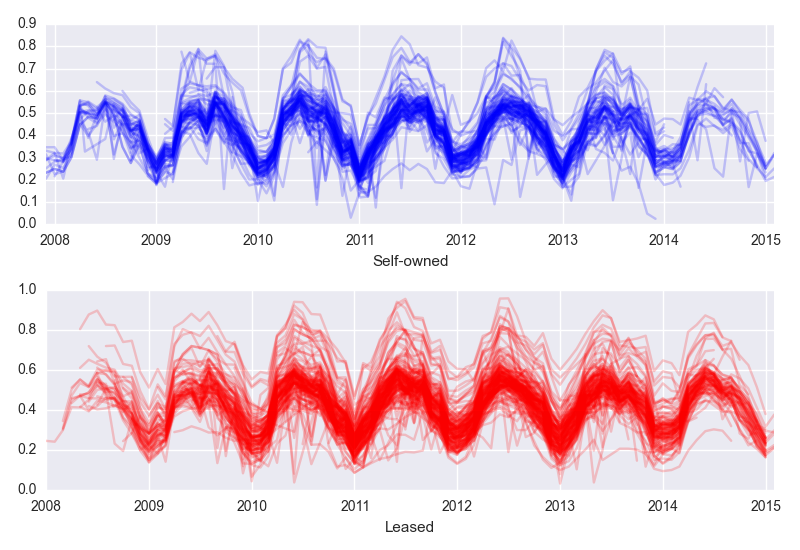
\includegraphics[width=1\textwidth]{tot_production.png}
	\caption{Production over time from California solar panels, Host owned and leased. Production index reflects monthly production in kWh normalized by capacity multiplied by 30.5*12 to reflect a rough estimate of maximum day-light hours in a month.}
	\label{tot_production}
\end{figure}

The main methodological goal of this paper is to make an unbiased estimate of the slope of the average degradation of solar panels - comparing the slopes between groups of systems that are leased and bought outright. These estimates should also control for seasonality and idiosyncratic factors between solar power systems.
A simple example of fitting a straight lines through two production series is shown in figure \ref{example_prod} - here as a simple single variable OLS estimate.

\begin{figure}
	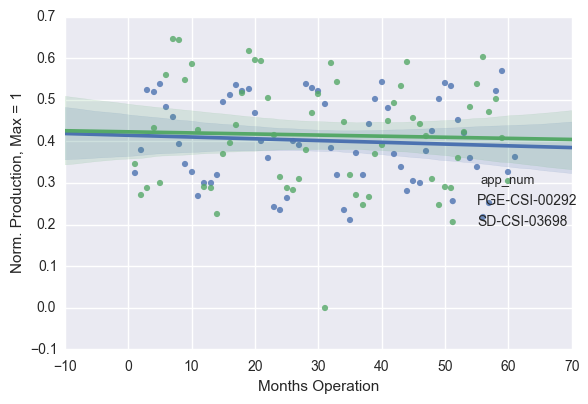
\includegraphics[width=1\textwidth]{example_prod.png}
	\caption{The main methodological task in this paper is to make an unbiased estimate of the slope of the average degradation of production over time. The figure demonstrates a straight line fitted to a time series from a single solar power system.}
	\label{example_prod}
\end{figure}

The question of interest and the structure of the available data suggests a hierarchical structure to the empirical model. The individual production data are grouped by the different solar panel systems. Each system is then in turn grouped into categories of leased or host-owned. As mentioned, seasonality must also be adequately accounted for as well as other factors such as geographic location, use of tracking and idiosyncratic variation from one solar panel system to another.

For later comparison, consider results from a traditional single-level regression of production over time estimated by maximum likelihood shown in table \ref{table:max_likelihood}. Fixed effects are included for month, host sector, county\footnote{coefficients for county are not shown}, and an indicator variable for leased systems. Variables for year of installation and size of the system are also included. The variable of interest is the interaction of the lease indicator with the time variable - which is transformed from monthly to fractional year units.

The results indicate a good fit with an $R^2$ of 90 percent. The coefficient of interest indicates that leased systems show 4\% less degradation over time than those sold outright - with a p-value of .001. However, even with the relatively large number of fixed effects included in this regression, much of the idiosyncratic variation from one photovoltaic system to another is not accounted for. I will show that when the full idiosyncratic variation is better accounted for, the evidence for a substantial difference in performance over time between leased and systems sold outright is substantially weaker than the below regression results indicate.

\begin{table}
\begin{center}
\begin{tabular}{l c }
\hline
 & Maximum Likelihood Results\\
\hline
(Intercept)                                            & $8.62^{***}$  \\
                                                       & $(0.08)$      \\
I(months\_operation/12)                                & $-0.03^{***}$ \\
                                                       & $(0.00)$      \\
Leased                         & $0.19^{***}$  \\
                                                       & $(0.01)$      \\
sys\_size\_dc                                          & $0.00^{***}$  \\
                                                       & $(0.00)$      \\        & $(0.08)$      \\
February                                         & $0.14^{***}$  \\
                                                       & $(0.02)$      \\
March                                        & $0.27^{***}$  \\
                                                       & $(0.02)$      \\
April                                        & $0.59^{***}$  \\
                                                       & $(0.02)$      \\
May                                         & $0.70^{***}$  \\
                                                       & $(0.02)$      \\
June                                         & $0.79^{***}$  \\
                                                       & $(0.02)$      \\
July                                         & $0.75^{***}$  \\
                                                       & $(0.02)$      \\
August                                         & $0.70^{***}$  \\
                                                       & $(0.02)$      \\
September                                         & $0.69^{***}$  \\
                                                       & $(0.02)$      \\
October                                       & $0.54^{***}$  \\
                                                       & $(0.01)$      \\
November                                       & $0.41^{***}$  \\
                                                       & $(0.01)$      \\
December                                        & $0.15^{***}$  \\
                                                       & $(0.01)$      \\
Fixed Array                            & $-0.52^{***}$ \\
                                                       & $(0.03)$      \\
Mixed                                  & $-0.34^{***}$ \\
                                                       & $(0.06)$      \\
Single-Axis Tracker                    & $-0.31^{***}$ \\
                                                       & $(0.04)$      \\
Government                               & $0.07^{***}$  \\
                                                       & $(0.01)$      \\
Non-Profit                               & $-0.17^{***}$ \\
                                                       & $(0.02)$      \\
Residential                              & $-2.12^{***}$ \\
                                                       & $(0.01)$      \\
I(months\_operation/12):leased & $0.04^{***}$  \\
                                                       & $(0.01)$      \\
\hline
R$^2$                                                  & 0.90          \\
Adj. R$^2$                                             & 0.90          \\
Num. obs.                                              & 32979         \\
RMSE                                                   & 0.57          \\
\hline
\multicolumn{2}{l}{\scriptsize{$^{***}p<0.001$, $^{**}p<0.01$, $^*p<0.05$}}
\end{tabular}
\caption{Results from a standard linear regression model with fixed effects for }
\label{table:max_likelihood}
\end{center}
\end{table}

Instead of standard single-level maximum likelihood estimation,  I use a hierarchical Bayesian model where parameters can be estimated through Markov Chain Monte Carlo (MCMC) simulation techniques. The main advantage of such models are the flexibility of taking into account the multi-level structure of the data and improved inference that comes from partial pooling.

Consider first a no pooling model. The slope of production over time from each solar panel system would be estimated independently - allowing for large amounts of solar-power-system level variance, but excluding information from data on all the other plants from each of the individual system-level inferences. On the other hand, in a fully pooled model, the data from all of the observations of all the solar power systems in each group (leased, sold outright) are used in the estimation, but idiosyncratic variation between solar-power-systems are not taken into account. An outlying solar power system may, for instance, have too much influence and bias the results.

A hierarchical model with partial pooling is a compromise between these two extremes. Individual estimators of the solar-power-system slopes make use of the information in the full dataset with weights established by the relative variance between and within solar power systems. A full discussion of partial pooling can be found in \citet{gelman_bayesian_2013} or \citet{kruschke_doing_2014}.


Figure \ref{solar_prod_bayes_diag} shows the structure of the model. Starting from the bottom, the individual production data are log transformed and modeled as having a Cauchy distribution with mean $y_hat$ and variance $sigma^2$. $sigma^2$ is in turn given a half-Cauchy prior.

The use of the Cauchy and half-Cauchy distribution reflects that a large in magnitude effect of around 5 or greater on the logit scale is highly unlikely in logistic regressions where all non-binary data has been transformed to have mean zero and standard deviation 1 - which I have done. In addition, the Cauchy distribution will give answers even under complete separation, and avoids computational problems inherent in assigning completely non-informative priors in multilevel models \citep{gelman_weakly_2008}.

Going up a level, $y_hat$ is modeled as having random group-level intercepts $\beta_{0,j}$, where j represents the j-th of $J$ solar panel system. The $\beta_{0,j}s$ are in turn modeled as function of system size, county, whether solar trackers are used, and a random effects term $re_j^0$.

In a similar manner the J $B_j$ coefficients are modeled as a function of whether the system is leased, $\mu_{lease}^1$, the host sector of the installation, the county, use of tracking, installation year and a random effects term $re^1_j$.  The question of interest - whether leased solar systems display a lower degree of degradation over time than those sold outright - can then be expressed as the distribution of the difference of the $mu_{lease}$ parameters: $\mu_{lease=1} - \mu_{lease=0}$.

Finally, to take into account the seasonality of the monthly data, random effects for each of the 12 months are estimated with a $Cauchy(0,4)$ prior on each parameter. The remaining hyper-parameters are given Cauchy or half-Cauchy priors.

\begin{figure}
	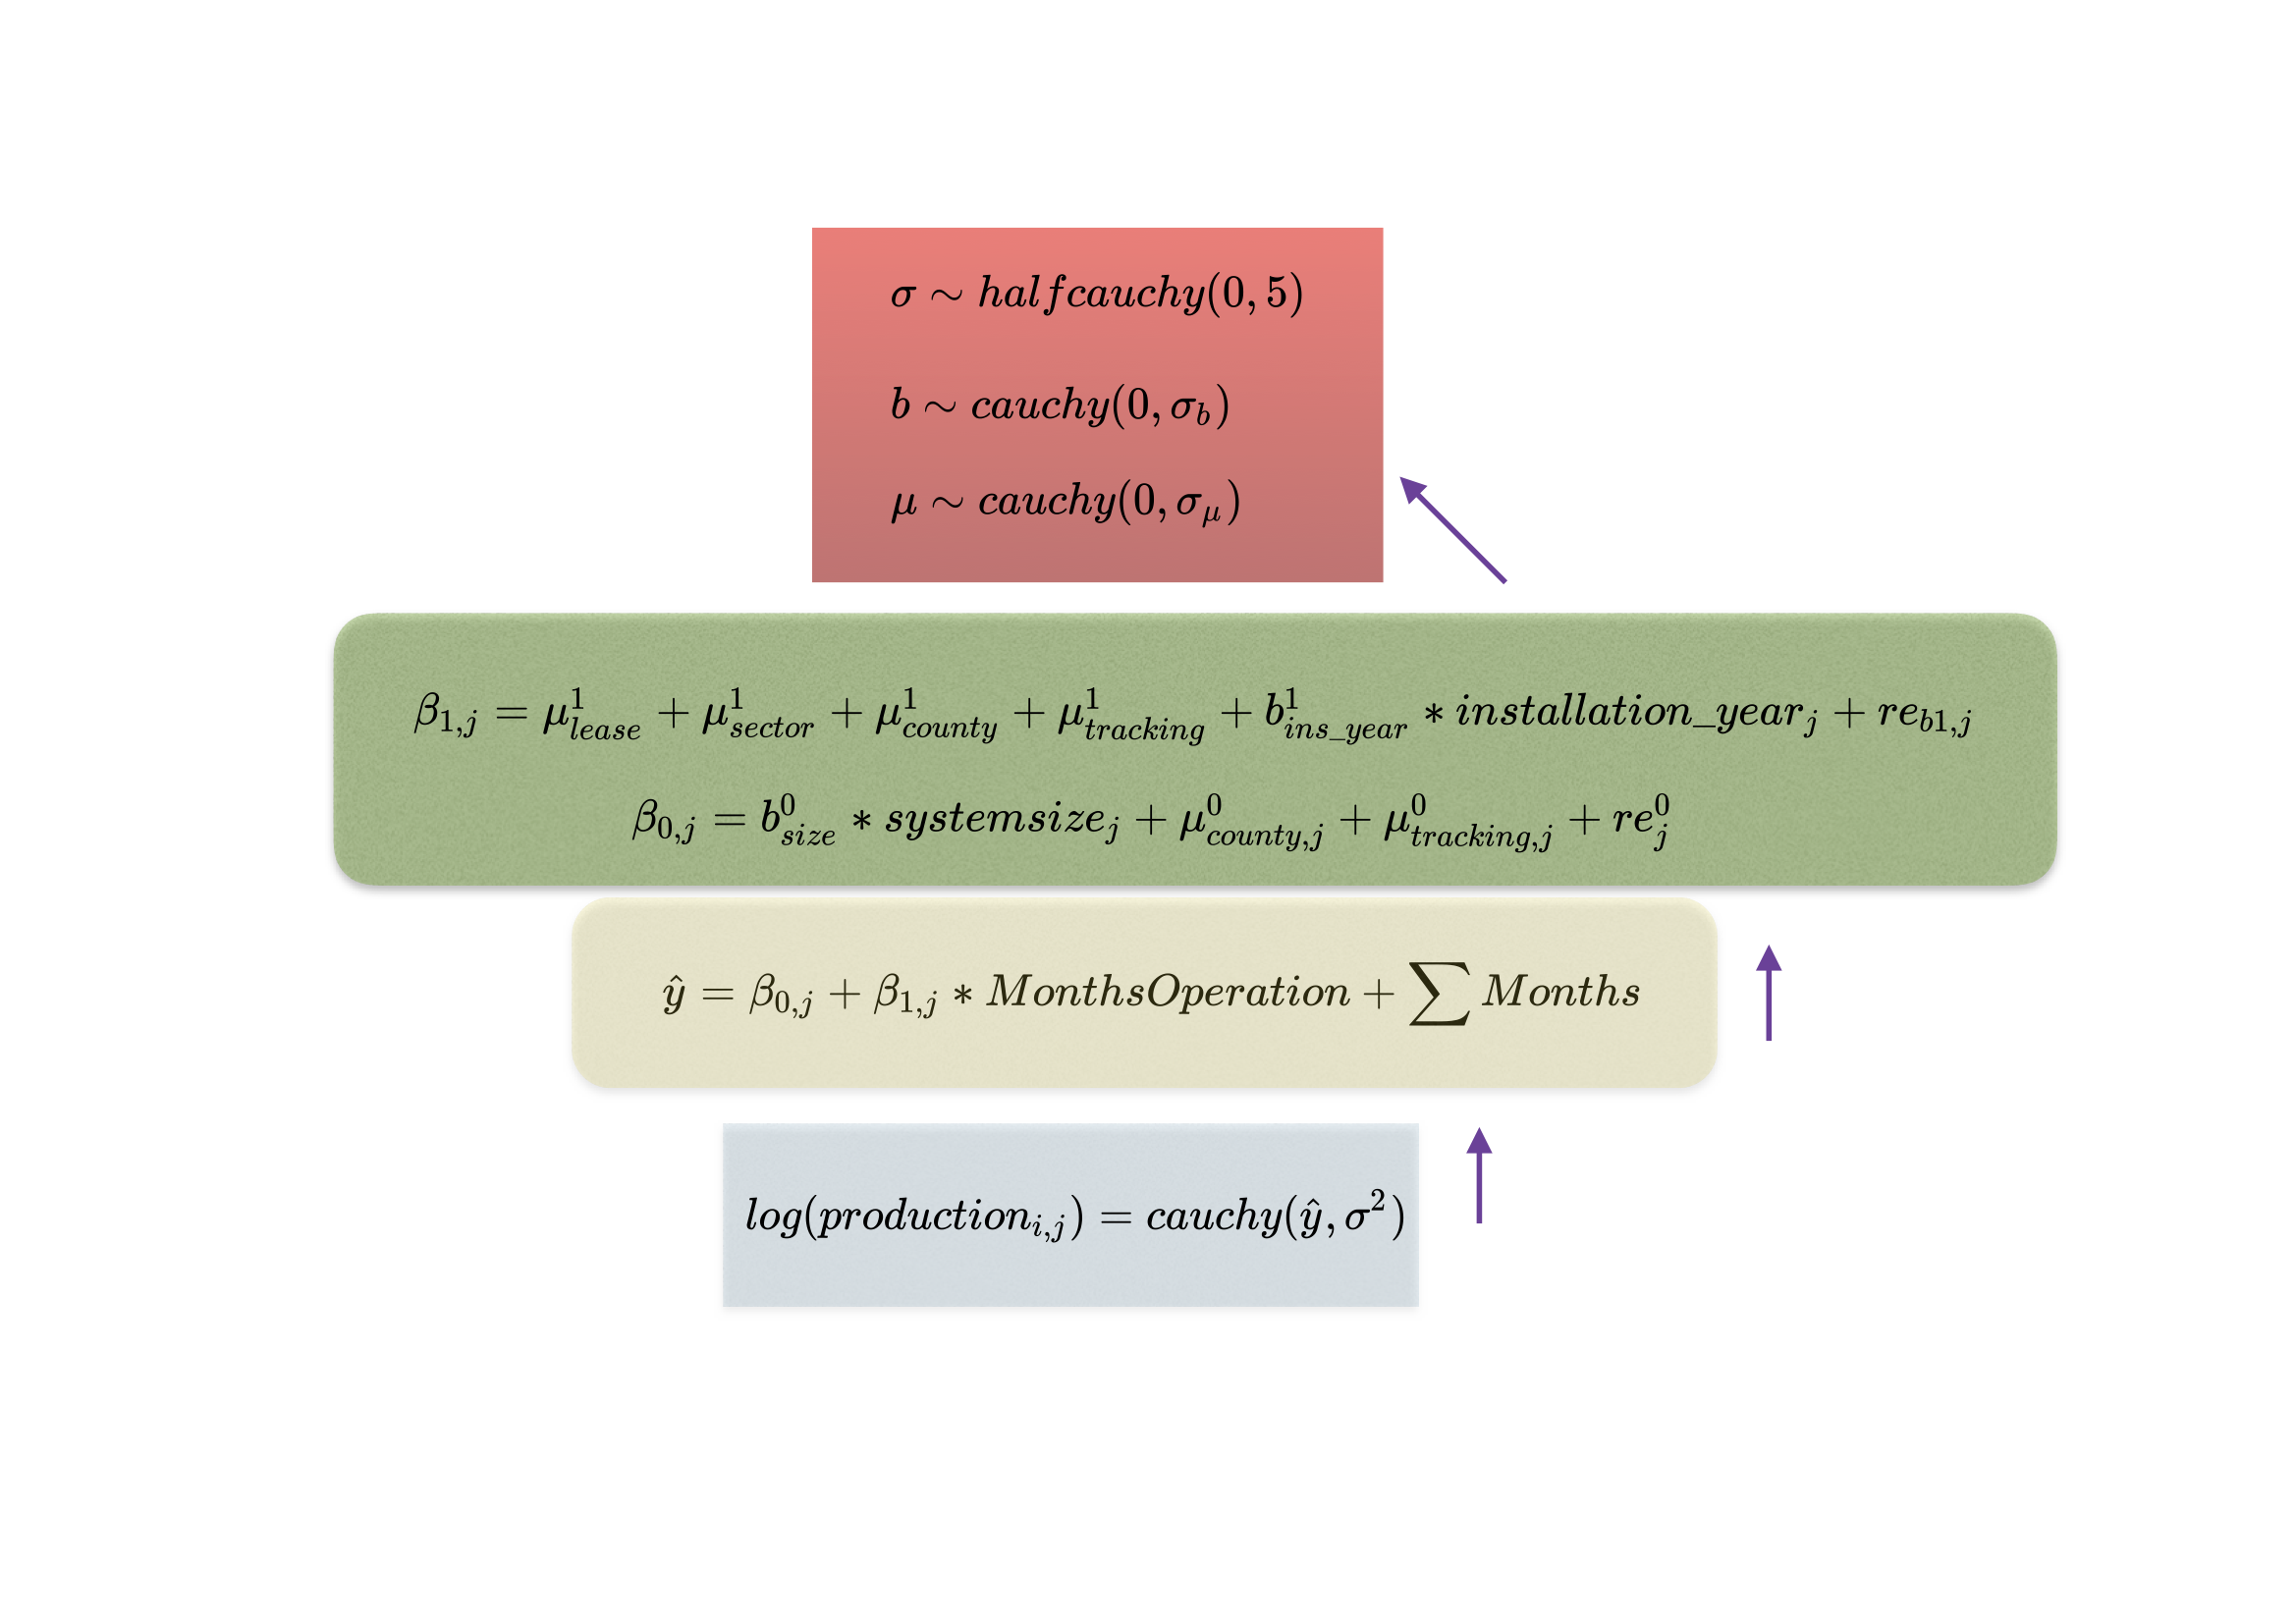
\includegraphics[width=1\textwidth]{figures/solar_prod_bayes_diag.png}
	\caption{The data and the research question combined suggest a hierarchical Bayesian model. The figure shows the structure of the model. Production data is grouped by individual solar panel systems (index i).}
	\label{solar_prod_bayes_diag}
\end{figure}

To estimate the parameters of the model, I use the Stan Bayesian programming language and simulator \citep{stan_development_team_stan_2014} which uses Hamiltonian MCMC to estimate a joint posterior distribution of the parameters. \citet{kruschke_doing_2014} provides an accessible explanation of the Hamiltonian MCMC algorithm, while more detailed technical descriptions are provided by \citet{gelman_bayesian_2013} and \citet{stan_development_team_stan_2014}.

Bayesian simulation methods are still emerging - especially in Economics. So it is worth spending a moment to motivate their use in this case over more common asymptotic methods. As mentioned, the main reason for using the Bayesian model is the flexible treatment it allows for modeling the inherent hierarchy of the data and allowing for partial pooling in estimation.

The usefulness of Bayesian models is most apparent in the estimation of complex hierarchical models with many parameters.
In a hierarchical model, lower-level parameters within a certain group are themselves modeled as coming from a distribution characterized by ``meta-parameters''. Thus, the estimated group-level parameters are a weighted function of both the observations within the group as well as the full set of observations in the dataset. For example, the estimated mean parameter on a group with a few, outlying observations would be pulled towards the full sample mean. This partial pooling also serves as a natural form of parameter shrinkage, which mostly eliminates the need for using corrections for multiple comparisons in inference \citep{gelman_data_2006}.

With Bayesian multilevel model, I also have greater flexibility in specifying the model without having to rely on assumptions like constant group-level variances and a Gaussian noise distribution.  Because Bayesian simulation techniques result in an estimate of the full joint probability distribution of the model, the inference has the potential to be more informative than the typical point estimates and p-values of of the standard hypothesis testing frameworks \citep{kruschke_doing_2014}.

Another advantage is that the posterior distributions of the parameters have a natural and direct interpretation as probabilities, as opposed to standard hypothesis testing where the concepts of p-values and significance are often ill-defined. See \citet{kruschke_doing_2014} or \citet{gelman_bayesian_2013} for further discussion.


% \begin{align}
% 		log(production_{ij}) &\sim N(\hat{y}, \sigma^2), \quad i=1,...,n \\
% 		\hat{y} &= \beta_{0j} + \beta_{1j}*time_{ij} + month_{m}
% 		\beta_{1,j} &= \mu_{\beta, l} + \zeta_{b1, j}, \quad j=1...j, \quad l = 0,1 \\
% 		\mu_{\beta1, l} &\sim N(0,10) \\
% 		\beta_{0,j} &\sim N(\mu_{b0}, \sigma_{b0}) \\
% 		\month_{m} &\sim N(1,10)\\
% 		\sigma &\sim uniform(0,100) \\
% 		\zeta_{b1, j} &\sim N(0,\sigma_{b1})
% 		\label{equation:model}
% 		\caption{}
% \end{align}

\section{Results}

I run 1000 iterations with 4 chains of the Hamiltonian MCMC algorithm in order to sample the joint posterior probability distribution of the model. I can then extract the the estimates of the marginal posterior distributions of the individual parameters in the form of a list of simulated parameter estimates.

Summary statistics for the posterior distributions of the main parameters of the model are shown in table \ref{table_results}. The parameters of interest are $\mu_{own}, \mu_{lease}$ which are the average slope of production over time in, respectively, systems that were sold outright and systems that were leased. These coefficients as well as the other component coefficients of $\beta1$, should be interpreted for a marginal change of 1 standard deviation change in time. Intuitive illustrations of the magnitudes of the coefficients of interest are shown further below.

\begin{table}
\resizebox{12cm}{!} {
\begin{tabular}{lrrrr}
\toprule
{} &  2.5\%&   97.5\% &   mean &  median \\
params           &          &          &         &          \\
\midrule
apr              &   0.1452 &  -0.0838 &  0.0069 &  -0.0013 \\
aug              &   0.2065 &  -0.0223 &  0.0681 &   0.0594 \\
dec              &  -0.1005 &  -0.3295 & -0.2386 &  -0.2471 \\
feb              &  -0.1037 &  -0.3346 & -0.2437 &  -0.2523 \\
jan              &  -0.1935 &  -0.4234 & -0.3319 &  -0.3404 \\
jul              &   0.2364 &   0.0058 &  0.0968 &   0.0886 \\
jun              &   0.2584 &   0.0282 &  0.1191 &   0.1105 \\
mar              &  -0.0257 &  -0.2535 & -0.1631 &  -0.1717 \\
may              &   0.2067 &  -0.0225 &  0.0687 &   0.0602 \\
nov              &   0.0546 &  -0.1748 & -0.0839 &  -0.0923 \\
oct              &   0.1256 &  -0.1034 & -0.0124 &  -0.0211 \\
sep              &   0.2094 &  -0.0205 &  0.0704 &   0.0619 \\
mu1\_commercial   &   0.0014 &  -0.0041 & -0.0007 &  -0.0005 \\
mu1\_government   &   0.0035 &  -0.0026 &  0.0004 &   0.0002 \\
mu1\_non\_profit   &   0.0018 &  -0.0057 & -0.0008 &  -0.0003 \\
mu1\_not\_tracking &   0.0044 &  -0.0074 & -0.0016 &  -0.0009 \\
mu1\_residential  &   0.0039 &  -0.0023 &  0.0005 &   0.0003 \\
mu1\_tracking     &   0.0039 &  -0.0092 & -0.0021 &  -0.0014 \\
mu\_lease         &  -0.0001 &  -0.0115 & -0.0045 &  -0.0042 \\
mu\_own           &  -0.0001 &  -0.0125 & -0.0054 &  -0.0054 \\
beta0\_size       &   0.7501 &   0.6948 &  0.7173 &   0.7141 \\
beta1\_ins\_year   &  -0.0007 &  -0.0032 & -0.0020 &  -0.0020 \\
beta1\_size       &  51.1251 & -45.7583 &  0.1312 &   0.0594 \\
sigma            &   0.0295 &   0.0287 &  0.0291 &   0.0291 \\
\bottomrule
\end{tabular}
}
\label{table_results}
\caption{Summary statistics of the distributions over the main parameters in the model. Confidence intervals are estimated as quantiles at 2.5 and 97.5 percent of the estimated posterior distribution of the parameters.}
\end{table}

I display the histograms representing the posterior distributions of these two parameters in the top panel of figure \ref{diff_lease}. The histograms indicate that the posterior distributions appear to have means that are different from each other.

In the lower panel, I show a histogram of the posterior of the difference between the two parameters, $\mu_{b1,l=1} - \mu_{b1,l=2} $ which is the direct test of the question of interest. 95\% of the probability lies below the vertical line, which stands at approximately zero. A direct interpretation is then that there is a 95 \% probability that on average solar power systems that are sold outright have a higher rate of degradation than those that are leased.

\begin{figure}
	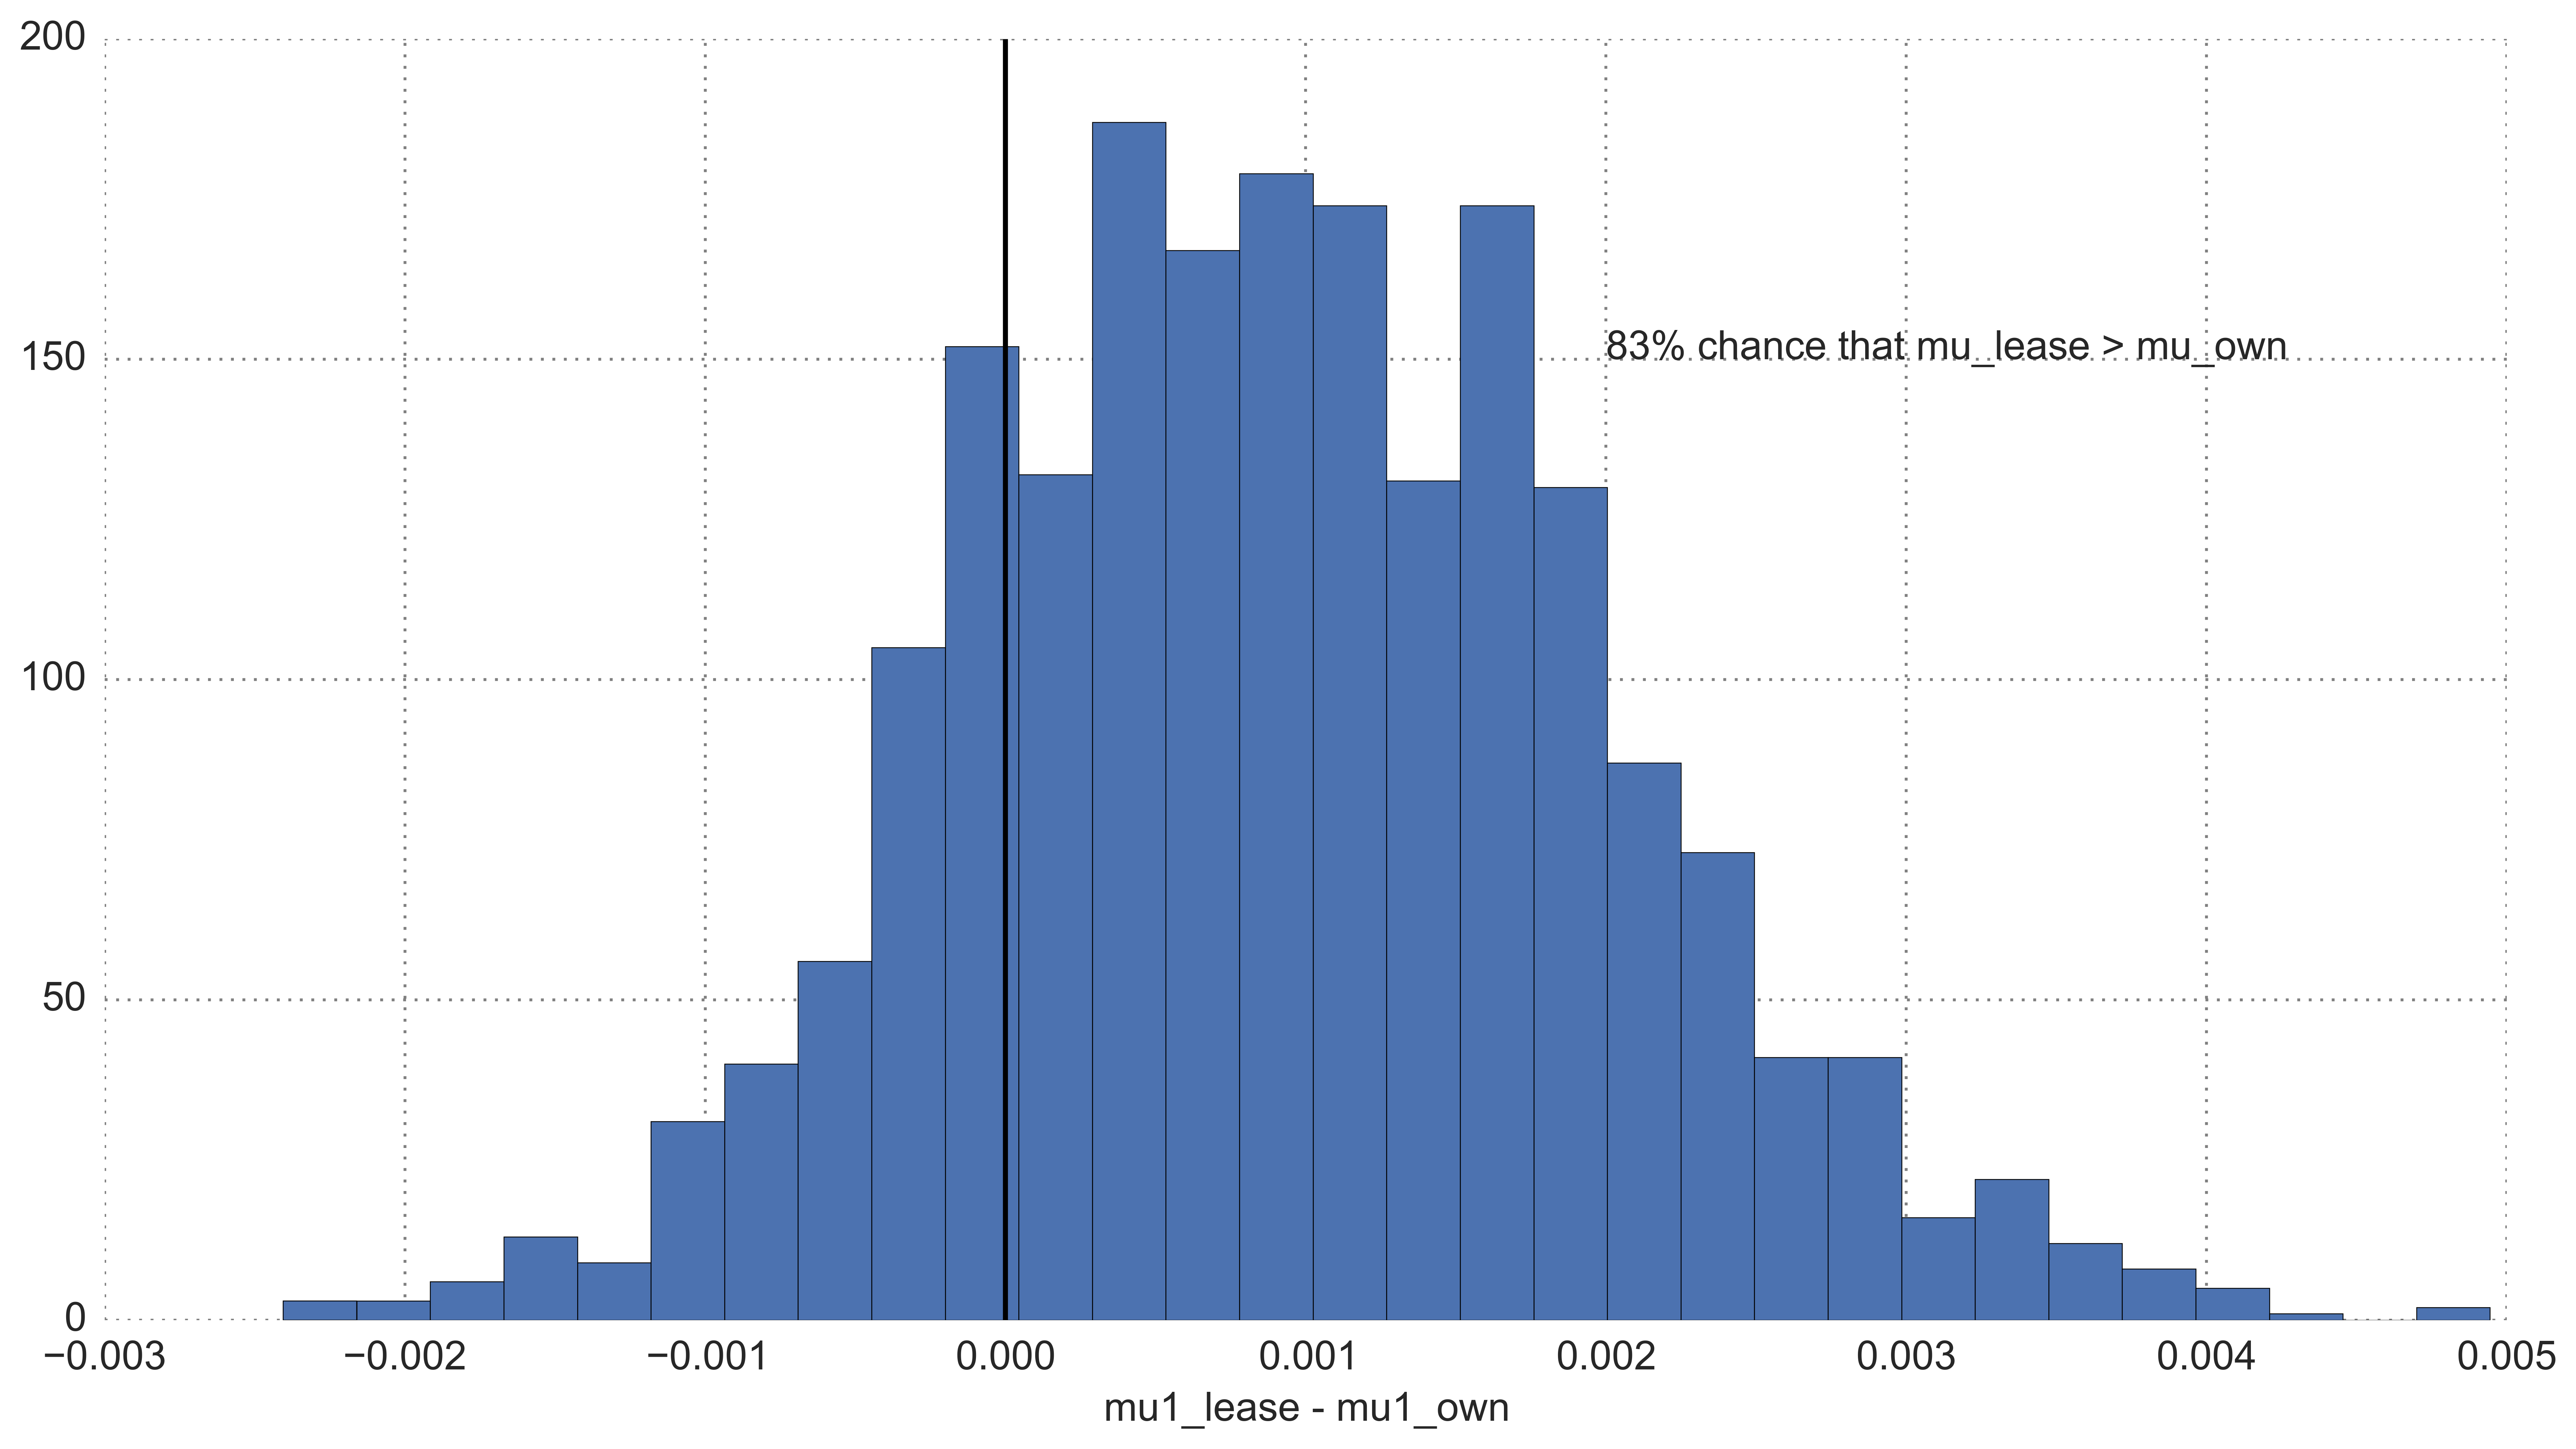
\includegraphics[width=1\textwidth]{figures/diff_lease.png}
	\caption{The figure shows the distribution of the difference of $\mu_{lease}$ and $\mu_{own} $. The black vertical line is placed at zero. The distribution of the difference of the two parameters suggests that leased panels had about a 80\% chance of being higher quality than those sold outright, as measured by the slope of production over time.}
	\label{diff_lease}
\end{figure}

The magnitude of the effect can best be seen by plotting average predicted values over time, which are shown for systems that are leased and sold-outright in figure \ref{predicted_deg}. The solid lines represent the median value of the posterior distribution on the $mu_lease$ and $mu_old$ parameters, where the light lines represent random draws from the respective posterior distributions to represent uncertainty. The model suggests that a leased solar panel system will on average experience degradation of about 6\% after 20 years while those owned outright experience on average of 5\% of degradation. However, as the figure makes clear, the average values hide significant variation in the overall distribution.

\begin{figure}
	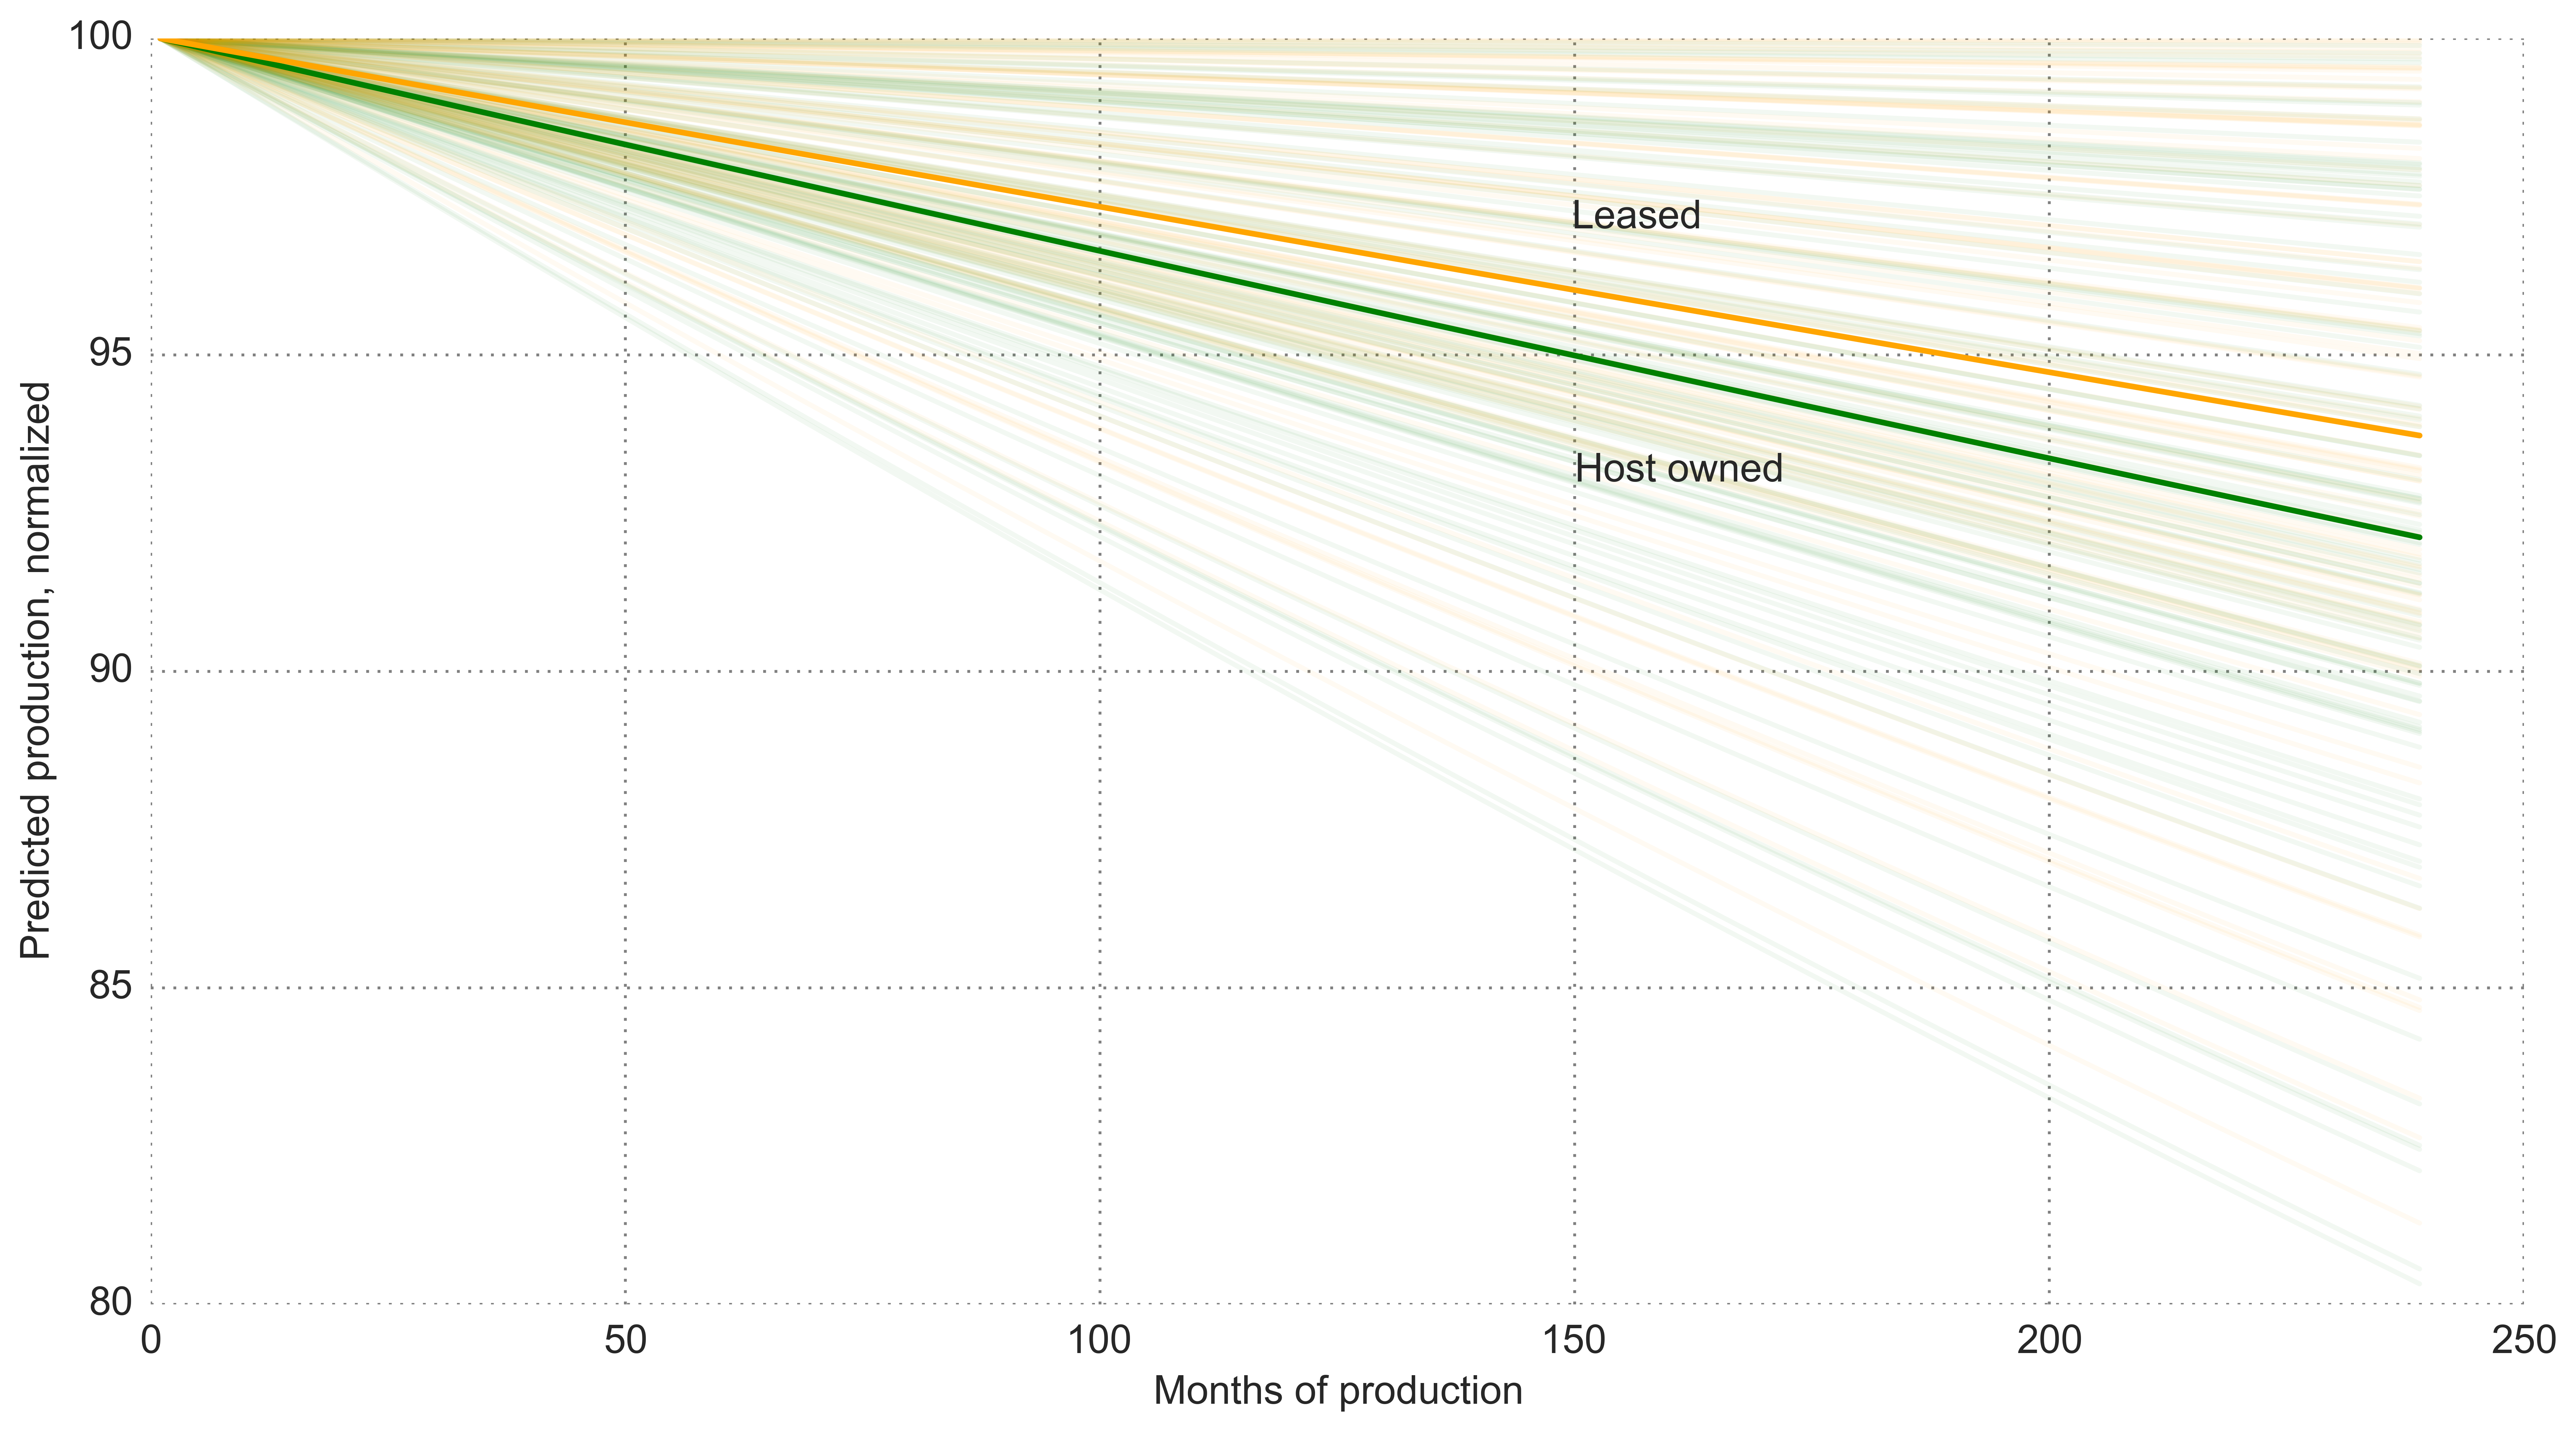
\includegraphics[width=1\textwidth]{figures/predicted_deg.png}
	\caption{The figure shows the average predicted values of degradation over time of solar panel systems that are leased and sold out-right. The solid lines represent the mean value of the posterior where the lighter lines represent random draws from the posterior distribution}
	\label{predicted_deg}
\end{figure}

\section{Discussion and Conclusion}
The theoretical literature on information asymmetry and quality is established and deep. The empirical literature for consumer durable investments is, however, more sparse, reflecting the difficulty of getting reliable data on purchases and long-term reliability. This article provides one of few case studies that both identifies a market that could be expected to have issues of information asymmetry of quality, and provides an indirect empirical test for the presence of information asymmetry of quality.

The structure of the emerging solar industry in the US, as well as other parts of the world suggests that issues of information asymmetry may play an important role. The established theory on the subject suggests that under information asymmetry of quality, poor quality products may push out good quality products, at least in some sub-markets. In this article I have tested an implication of that theory for the case of solar panels in California. The results provide some weak evidence for the existence of information asymmetry issues of quality.

The use of Bayesian MCMC simulation techniques in this article also provides an illustrative example of the use and usefullnes of a powerful emerging toolset. The Bayesian frameworks and recently developed software such as Stan provide major practical and theoretical advantages over many traditional econometric methods. These methods and tools are also increasingly accessible to the practicioner. \citet{kruschke_doing_2014} and \citet{stan_development_team_stan_2014} provide accessible and thorough introductions and guides.

This article should also be considered as part of a broader literature on the special characteristics of new distributed energy generation technologies. The energy investment behavior of home owners, farmers, and small cooperatives are bound to be substantially different than those of large, specialized energy companies that have traditionally done most of the investment in electricity generation. Understanding the quickly evolving energy and power industry requires taking into account informational and behavioral factors, and this is a rich field for further research

\begin{spacing}{1}
\bibliographystyle{plainnat}
\bibliography{solar_prod}

\FloatBarrier

\appendix
\section{Appendix: Tables}


\end{spacing}
\end{document}
